% This is LLNCS.DEM the demonstration file of
% the LaTeX macro package from Springer-Verlag
% for Lecture Notes in Computer Science,
% version 2.4 for LaTeX2e as of 16. April 2010
%
\documentclass{llncs}
%
\usepackage{makeidx}  % allows for indexgeneration
%
\usepackage[misc]{ifsym}
\usepackage{graphicx}
\usepackage{multirow}
\usepackage{float}
\usepackage{listings}
\usepackage{color}	

\definecolor{dkgreen}{rgb}{0,0.6,0}
\definecolor{gray}{rgb}{0.5,0.5,0.5}
\definecolor{mauve}{rgb}{0.58,0,0.82}

\lstset{frame=tb,
  language=Python,
  aboveskip=3mm,
  belowskip=3mm,
  showstringspaces=false,
  columns=flexible,
  basicstyle={\small\ttfamily},
  numbers=none,
  numberstyle=\tiny\color{gray},
  keywordstyle=\color{blue},
  commentstyle=\color{dkgreen},
  stringstyle=\color{mauve},
  breaklines=true,
  breakatwhitespace=true,
  tabsize=3
}

%
\begin{document}
%
\frontmatter          % for the preliminaries
%
\pagestyle{headings}  % switches on printing of running heads
\addtocmark{Hamiltonian Mechanics} % additional mark in the TOC
%
\title{An Improvement of PyMIC for Deep Learning Application on Intel Xeon Phi}
%
\titlerunning{pyMIC2}  % abbreviated title (for running head)
%                                     also used for the TOC unless
%                                     \toctitle is used
%
\author{Anh-Tu Ngoc Tran\textsuperscript{(\Letter)} \and
Phu  \and
Tri Nguyen Minh \and
Thanh-Dang Diep \orcidID{0000-0003-1163-7464} \and
Hung \and
Nam Thoai
}
%
\authorrunning{Ivar Ekeland et al.} % abbreviated author list (for running head)
%
	%%%% list of authors for the TOC (use if author list has to be modified)
\tocauthor{Ivar Ekeland, Roger Temam, Jeffrey Dean, David Grove,
Craig Chambers, Kim B. Bruce, and Elisa Bertino}
%
\institute{Faculty of Computer Science and Engineering\\ HCMC University of Technology, VNUHCM, Vietnam\\
\email{\{51304672,51302990,...\}@hcmut.edu.vn},\\ %WWW home page:
%\texttt{http://users/\homedir iekeland/web/welcome.html}
%\and
%Universit\'{e} de Paris-Sud,
%Laboratoire d'Analyse Num\'{e}rique, B\^{a}timent 425,\\
%F-91405 Orsay Cedex, France
}

\maketitle              % typeset the title of the contribution

\begin{abstract}
The abstract should summarize the contents of the paper
using at least 70 and at most 150 words. It will be set in 9-point
font size and be inset 1.0 cm from the right and left margins.
There will be two blank lines before and after the Abstract. \dots
Deep learning plays a vital role in a broad spectrum of scientific fields such as computer vision, speech recognition and natural language processing and so on. In order to support deep learning, many frameworks are created with the aim of setting up artificial neural networks as quickly as possible. Such frameworks can be run on systems including either Graphical Processing Unit or Intel Xeon Phi the second generation - Knights Landing coprocessor. In addition, few deep learning frameworks can be run on legacy systems containing Intel Xeon Phi Knights Corner. For that reason, we propose and develop pyMIC2 which is a NumPy-like library supporting deep learning frameworks run on such legacy systems. pyMIC2 that is an extension of offloading module pyMIC implements basic functions so that it can be integrated easily into deep learning frameworks. The experimental findings show that pyMIC2 outperforms NumPy in terms of two hardware platform with the same theoretical performance. Moreover, pyMIC2 shows it is highly effective when integrating it into a well-known deep learning framework Chainer with very impressive performance. Hence, pyMIC2 is a fairly promising NumPy-like library to facilitate deep learning frameworks run on the legacy systems.

\keywords{computational geometry, graph theory, Hamilton cycles}
\end{abstract}
%
\section{Introduction, 2 pages}
%
With this chapter, the preliminaries are over, and we begin the search
for periodic solutions to Hamiltonian systems. All this will be done in
the convex case; that is, we shall study the boundary-value problem
Deep Learning has proliferated over the last decade because of its very profound impact on a wide range of several application areas, namely computer vision[x], speech recognition[x], and natural language processing[x]. In order to put research ideas into practice, advances in deep learning frameworks are a considerable need for the implementation of artificial neural networks (ANNs). Therefore, some frameworks are developed to meet the need, such as Caffe, TensorFlow, Theano, Torch and so on. 

Recent years have witnessed a rapid growth of High Performance Computing field with the advent of new high-end supercomputers which have incredible computational power [x]. Most of the supercomputers take advantage of accelerators, such as Graphic Processing Unit (GPU) or Intel Xeon Phi coprocessor. In addition, most researchers and programmers run deep learning applications on systems consisting of GPU. There are just a few deep learning frameworks, like Caffe, TensorFlow, Theano and Neon[x], which can currently be run on infrastructure including Intel Xeon Phi coprocessor. Unfortunately, the frameworks can only be run on systems including Intel Xeon Phi Knights Landing but not for Knights Corner. Consequently, few deep learning frameworks can be run on several legacy systems, such as Tiane-2 (MilkyWay-2), Thunder, cascade and so forth. This leads to the fact that it is difficult to exploit fully computational power of the underlying hardware platform in case it is not in use. For that reason, the need for developing a novel framework which can be run on such legacy systems is very significant. However, in this paper, our goal is to develop a flexible library which can straightforwardly be integrated into deep learning frameworks rather than a new deep learning one.

pyMIC [x] is a Python module for offloading compute kernels from a Python program to the Intel Xeon Phi Knights Corner coprocessor. Currently, it can simply be leveraged in several scientific computing applications, such as the Python-based open source electronic-structure simulation software GPAW[x] and the open-source high-order accurate computational fluid dynamics solver for unstructured grids PyFR [x]. In this paper, we present pyMIC2, the next generation of pyMIC with the aim of developing a library supporting Intel Xeon Phi Knights Corner coprocessor for deep learning frameworks. pyMIC2 is expanded from pyMIC by implementing functions similar to NumPy[x] to adapt it in order to deep learning frameworks by dint of flexible and layered characteristics of pyMIC. 

pyMIC2 mainly provides a myriad of NumPy-like rudimentary functions, like equal, or, abs, mean, sum and so on. Furthermore, pyMIC2 improves significantly several existing functions of pyMIC in the performance aspect via vectorization mechanism. The functions of pyMIC2 can directly be run on Intel Xeon Phi Knights Corner coprocessor by dint of offloading mechanism. Besides, they facilities high-level functions used as block buildings in establishment of ANNs, such as activate function, loss function, accuracy function and so forth.

We evaluate pyMIC2 with regard to two aspects: (1) discrepancy in performance in comparison with NumPy and (2) feasibility of pyMIC2 when integrating it into the well-known deep learning framework Chainer. Experimental results demonstrate that pyMIC2 outperforms NumPy in terms of computation time when considering them based on two different hardware platforms with same theoretical performance. Given such effectiveness of performance aspect, we conclude that pyMIC2 is a flexible but effective library which is highly integrated to deep learning frameworks.

In brief, this work makes the following contributions:
\begin{itemize}
\item We optimize several existing functions of pyMIC so as to increase program performance.
\item We implement pyMIC2 which is extended from pyMIC by means of implementing some numpy-like functions so that it can facilitate greatly several deep learning frameworks run on the legacy systems containing Intel Xeon Phi Knights Corner coprocessor. Therefore, researchers and programmers can closely integrate pyMIC2 into their interesting deep learning framework.
\item We try to integrate pyMIC2 into the well-known framework Chainer [x] and evaluate the effectiveness as well as flexibility of pyMIC2.
\end{itemize}

The remainder of the paper is organized as follows. The next section reviews in detail traditional vector clock techniques expressing the ordering of events in distributed systems. Section III properly formulates the system model considered in this literature while Section IV demonstrates a workable completed-before relation for MPI one-sided communication. A time-stamping system able to use in place with the concept of time for MPI one-sided communication is elaborated in Section V along with its implementation being depicted in Section VI. Finally, Section VII gives some conclusions and the further enhancement of the study.

\section{Background, 2 pages}
\subsection{MIC Architecture}

From the perspective of a developer, it is important to know features of MIC architecture if you want to optimize your applications so that it can run efficiently on Intel Xeon Phi. As your can see in figure \ref{fig:arch} \cite{phibook}, all processors and memory controllers are connected to a Core Ring Interconnect (CRI). Moreover, KNC has NUMA (non-uniform memory access) architecture which means that not all processors have equal access time to all memories.

\begin{figure}[h]
\centering
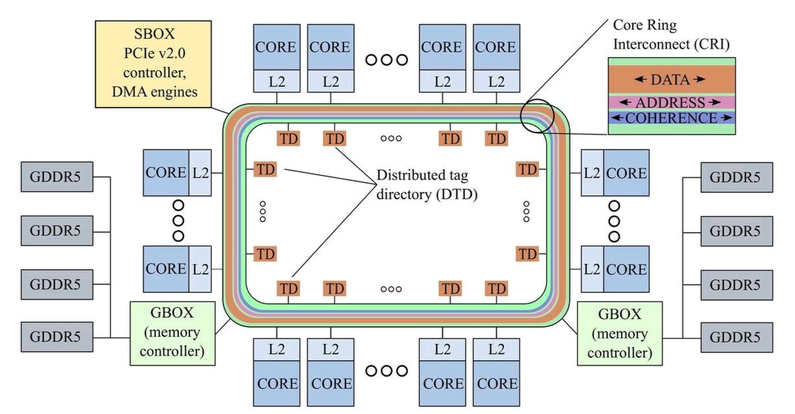
\includegraphics[scale=0.45]{img/mic-arch.png}
\caption{Knights Corner Architecture}
\label{fig:arch}
\end{figure}

KNC is equipped with 61 cores, each core can launch up to 4 hardware threads run in round-robin order. Vector unit, presents in each core, has 512-bit wide registers (vector registers). This functionality allows SIMD operations on up to 16 single precision floating-point numbers, or up to 8 double precision numbers. In terms of memory, KNC has a two-level cache hierarchy (cache level 1 32KB, level 2 512KB) for each core and from 6GB to 16GB shared memory depending on product series. Furthermore,GDDR5 memory can provide a bandwidth of 325GB/s per coprocessor. Of all hardware specifications mentioned above, theoretical peak performance of KNC is 1200 GFLOPS for double precision and 2400 GFLOPS for single precision.

\subsection{PyMIC}

For several recent years, Python has emerged as a popular scripting language in HPC thanks to its elegance, ease-to-program and ability to reduce development time and make flexible software. However, its convenience trades off for its performance in comparison in C which is a traditional language used in HPC. In 2012, Intel brought to the market a [?]coprocessor named Intel Xeon Phi with powerful computing ability and energy-efficient feature, but it only supports C/C++ and Fortran language. Therefore, the creation of PyMIC [ ] has helped to connect C code and Python code so that users can write Python application executed on Intel Xeon Phi (figure \ref{fig:pymic-feat}). To be specific,  PyMIC provides its API to invoke functions (also called kernels) written in C to execute on Intel Xeon Phi. Moreover, PyMIC is not only designed to be a bridge between two languages, its API is also compatible to Numpy, which is Python-API library for scientific computing. Data structures of Numpy can work with PyMIC without causing any conflict.

\begin{figure}[h]
\centering
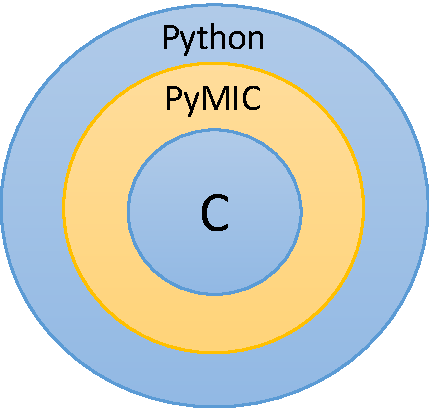
\includegraphics[scale=0.5]{img/pymic-feat.pdf}
\caption{PyMIC functionality}
\label{fig:pymic-feat}
\end{figure}

To provide an easy-to-use interface with slow overhead and full control over data transferring and offloading. Layered architecture of PyMIC is depicted in figure \ref{fig:pymic-arch}. In the lowest layer, Intel Language Extension for Offloading (Intel LEO) is responsible for directly interacting with coprocessor through compiler [?]pragmas or directives. In the higher layer, \_pyMICimpl is a Python extension module written in C/C++, and works as a connector between the highest layer (pyMIC) and the lowest one. To call C functions from pyMIC layer, \_pyMICimpl uses Cython mechanism. Besides, the key class of PyMIC is PyMIC also contains offload\_array class which is totally compatible with class ndarray of Numpy, and several standard kernel that implement array operations.		

\begin{figure}[h]
\centering
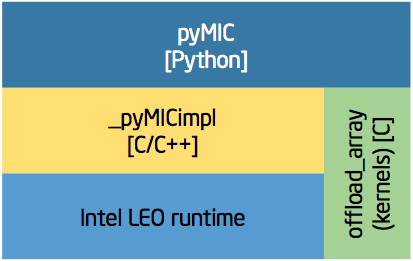
\includegraphics[scale=0.5]{img/pymic-arch.png}
\caption{Architecture of the pyMIC module}
\label{fig:pymic-arch}
\end{figure}

To better understand how PyMIC works, we consider the following example. In figure \ref{fig : Pymic dgemm }, first of all to use PyMIC in Python code, we import package \textbf{pymic}. PyMIC has  In line 5, Xeon Phi card 0 is selected through a global variable \textbf{device} to manage all Xeon Phi cards in a node. In the next line, a \textbf{stream} from that device is created, it functions as a queue to receive requests from host CPU. Kernel \textbf{mydgemm} written in C (figure \ref{fig : C dgemm}) will be compile by C compiler (can be Intel compiler or gcc) into a shared library \textbf{libdgemm.so}, it then is offloaded to device by Python API, which is described in line 7. In this example, we demonstrate a general matrix multiplication invoked from Python code. Input matrices are initialized  with random values by random function in Numpy package, while output matrix is filled with 0s. However, to do this operation on Xeon Phi, we first have to transfer data to coprocessor. From line 20 to 22, input arrays \textbf{a} and \textbf{b} are transfer to device by [?]enqueuing a request to \textbf{stream}. To be specific, a region of memory will be allocated and data will be copied from host to device. However, with output array \textbf{c}, we do not need to copy data to device by specifying \textbf{update\_device=False}. Transferring data between host and device is very costly; therefore, to achieve better performance, minimizing data movement is necessary. After transferring data to coprocessor, a computing kernel will be invoked by PyMIC API in line 25 and 26. In order to transfer data back to host CPU, member function \textbf{update\_host()} of \textbf{offload\_array} object will be called. In addition, all of functions related to data transferring and array manipulation are done completely asynchronously in chronological order of requests put in queue \textbf{stream}. Using \textbf{sync()} function  of \textbf{stream} in line 28 to wait until the queue is empty. In summary, figure \ref{fig:working mechanism} will gives you an overview of how PyMIC works.

\begin{figure}
    \centering
    \begin{lstlisting}
1  import pymic
2  import numpy as np
3
4  # select device and load kernel library
5  device = pymic.devices[0]
6  stream = device.get_default_stream()
7  library = device.load_library("libdgemm.so")
8
9  # size of the matrices
10 m, n, k = 4096, 4096, 4096
11
12 # create some input data
13 alpha = 1.0
14 beta = 0.0
15 a = np.random.random(m, k) 
16 b = np.random.random(k, n) 
17 c = np.zeros(m, n)
18
19 # create offloaded arrays
20 offl_a = stream.bind(a)
21 offl_b = stream.bind(b)
22 offl_c = stream.bind(c, update_device=False)
23
24 # perform the offload and wait for completion
25 stream.invoke(library.mydgemm,
26                  offl_a, offl_b, offl_c, m, n, k, alpha, beta)
27 offl_a.update_host()
28 stream.sync()
\end{lstlisting}
    \caption{PyMIC Python code example}  
    \label{fig : Pymic dgemm }
\end{figure}

\begin{figure}
    \centering
    \begin{lstlisting}[language=C++]
1  #include <pymic_kernel.h>
2  #include <mkl.h>
3
4  PYMIC_KERNEL
5  void mydgemm(const double *A, const double *B,
6               double *C,
7               const int64_t *m, const int64_t *n,
8               const int64_t *k,
9               const double *alpha,
10              const double *beta) {
11      /* invoke dgemm of MKL's cblas wrapper */
12     cblas_dgemm(CblasRowMajor, CblasNoTrans,
13                  CblasNoTrans,
14                  *m, *n, *k, *alpha, A,
15                  *k, B, *n, *beta, C, *n);
16 }
\end{lstlisting}
    \caption{PyMIC C code example}
    \label{fig : C dgemm}

\end{figure}

\begin{figure}[h]
\centering
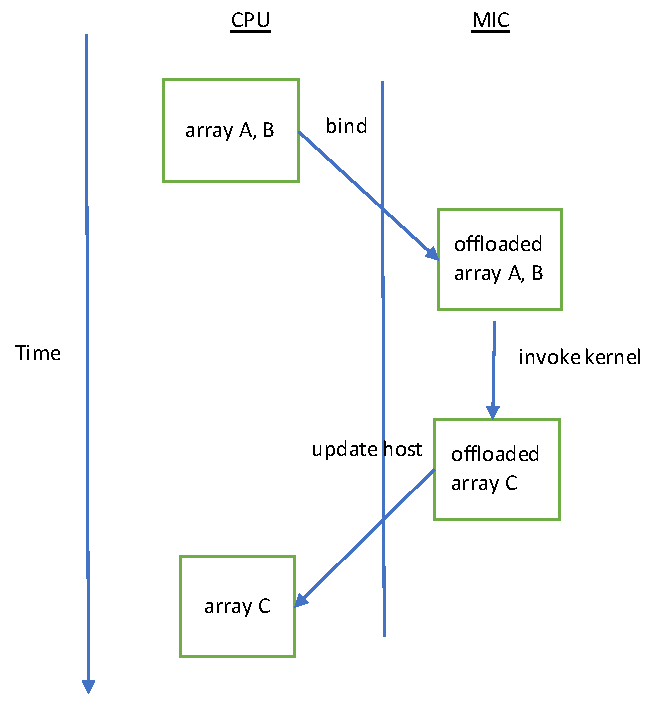
\includegraphics[scale=0.5]{img/working-mechanism.pdf}
\caption{PyMIC working mechanism}
\label{fig:working mechanism}
\end{figure}

\section{Implementation, 2 pages}
%table of function: name functionality, input, output
Let consider an example, we have an application with four computing functions and only implement 2 kernels written for the first function and the third one to be executed on coprocessor. As described in Fig. \ref{fig:working mechanism}, to execute the first function, data must be transfered to the coprocessor first and then taken back to host CPU after computation to be input for the second function. This process is repeated for the last two functions. We can see that, this application transfers data to coprocessor two times, and take it back to CPU times. However, data transferring leads to depletion in performance. Therefore, to minimize transferring time in this application, all functions must have corresponding kernels written to be offloaded to coprocessor. With this approach no matter there are how many functions in an application, we only spend one time to send data to coprocessor and one time to take the result back when all functions has finished. 

In the previous PyMIC version, it only provides several functions to initialize, change data in array and some simple operations on array such as add, subtract, multiply, and so on. In this paper, we enhance PyMIC by implementing all unit functions that mainly support for deep learning applications with high performance so that users do not have to spend time writing their own kernel. Our kernels are written in C code and parallelized by using OpenMP frameworks to make use of computing power of Intel Xeon Phi. Each unit function is implemented and designed in 3 steps:

\begin{itemize}
\item Defining function prototype for C kernel: In this step, we identify parameters needed to be input of a kernel, and their data types. Each parameter is a piece of data transferred to coprocessor; therefore, the number of parameters needs to be chosen wisely to achieve the best performance.

\item Implementing function in Python layer: function prototype in Python layer is the same as the one of Numpy so that users can easily use PyMIC in an application using Numpy if they want to execute their application on coprocessor without much modification because their function APIs are the same. The functionality of functions in this layer is to prepare parameters defined in previous step to transfer to kernels in C layer  		
			
\item Implementing function in C layer: After receiving input data from Python layer, C functions will do computation depending on input data types and return data back to Python layer. These kernels use data parallel algorithms which are implemented using \textbf{\#pragma omp simd} to take advantage of vector units, and \textbf{\#pragma omp for} to use up all core in Intel Xeon Phi
\end{itemize}


\section{Evaluation, 10 pages}
In this section, we demonstrate the performance of pyMIC2 by comparing functions implemented in pyMIC2 to those of NumPy. We then evaluate MNIST handwritten digit recognition application by using a deep learning framework called Chainer. This application is a classical one in machine learning. The core computing library of Chainer is NumPy, and we want to replace it with pyMIC2 to see how well pyMIC2 works in comparison to NumPy so that we can prove that our approach is practical and efficient enough. Before discussing all of that, we first consider the environment and system on which our experiments are conducted.

\subsection{System Setup}
In this paper, all of the experiments are conducted on a compute node that has 128 GB RAM, two-way processor Intel Xeon CPU E5-2680 v3 @ 2.50GHz about 1 TFLOPS and 2 first generation Intel Xeon Phi coprocessors 7120 series connected through PCIe with 1.2 TFLOPS each card.

Furthermore, in order to utilize all computing power of Intel Xeon Phi coprocessor, all threads must be used. However, threads can migrate from one core to another, which is depending on OS scheduling decisions. This leads to performance depletion because migrated threads must fetch data into cache of a new core \cite{colfaxbook}. Among all of the optimization techniques on Intel Xeon Phi, there is one called thread affinity. We can inhibit thread migration by setting environment variable KMP\_AFFINITY to scatter, compact, or several other modes \cite{threadaffinity}, and two of the most popular are scatter and compact. The former is especially good for memory and the latter is for computing.

Moreover, we can improve data transfer performance by using huge memory pages. When data offloaded to coprocessor exceed a threshold value set to MIC\_USE\_2MB\_BUFFERS, memory will be allocated on big 2MB pages, by default the size of pages on Intel Xeon Phi is 4KB. Therefore, we can access more data with less pages, which will decrease page fault rate \cite{bigmempage}. There is also a lower allocation cost.

%[https://software.intel.com/en-us/mkl-linux-developer-guide-improving-performance-on-intel-xeon-phi-coprocessors].

In summary, to achieve the best performance, our system is configured to KMP\_AFFINITY=compact, MIC\_USE\_2MB\_BUFFERS=16K. Additionally,  all of our benchmarks are run 100 times.

%, and any jitter will be removed to guarantee the accuracy of all benchmarks.

\subsection{Evaluation of computing functions in pyMIC2}
NumPy with easy-to-use Python API is a big, high performance computing library and has been developed and updated for a decade. In pyMIC2, we only implement several unit functions that mainly support deep learning. We divide these into three group (Table \ref{list-func}):
\begin{itemize}
	\item The first group is related to logical operations.
	\item The second group is about arithmetic, exponential and logarithmic functions. 
	\item The final group only consists of 1 function which is matrix multiplication function. This is a one of the important benchmarks in LINPACK used to measure the performance for a given machine.
\end{itemize}

%\begin{table}[]
%\centering
%\caption{My caption}
%\label{my-label}
%\begin{tabular}{|c|c|c|}
%\hline
%\multicolumn{2}{|c|}			{\multirow{4}{*}{Group 1}} 		& EQ \\ \cline{3-3} 
%\multicolumn{2}{|c|}{}                         				& GT \\ \cline{3-3} 
%\multicolumn{2}{|c|}{}                         				& NE \\ \cline{3-3} 
%\multicolumn{2}{|c|}{}                         				& OR \\ \hline
%\multirow{17}{*}{Group 2} 	& \multirow{9}{*}{Subgroup 1} 	& ABS \\ \cline{3-3}
%\multirow{17}{*}{} 			& \multirow{9}{*}{} 				& MEAN \\ \cline{3-3}
%\multirow{17}{*}{} 			& \multirow{9}{*}{} 				& SUM axis=0 \\ \cline{3-3}
%\multirow{17}{*}{} 			& \multirow{9}{*}{} 				& SUM axis=1 \\ \cline{3-3}
%\multirow{17}{*}{} 			& \multirow{9}{*}{} 				& SUM axis=None \\ \cline{3-3}
%\multirow{17}{*}{} 			& \multirow{9}{*}{} 				& ARGMAX axis=1 \\ \cline{3-3}
%\multirow{17}{*}{} 			& \multirow{9}{*}{} 				& ADD 2 shape-equal arrays  \\ \cline{3-3}
%\multirow{17}{*}{} 			& \multirow{9}{*}{} 				& SUB 2 shape-equal arrays\\ \cline{3-3}
%\multirow{17}{*}{} 			& \multirow{9}{*}{} 				& MUL 2 shape-equal arrays \\ \cline{2-3}
%\multirow{17}{*}{} 			& \multirow{5}{*}{Subgroup 2} 	& ARANGE \\ \cline{3-3}
%\multirow{17}{*}{} 			& \multirow{5}{*}{} 				& MAXIMUM \\ \cline{3-3}
%\multirow{17}{*}{} 			& \multirow{5}{*}{} 				& LOG \\ \cline{3-3}
%\multirow{17}{*}{} 			& \multirow{5}{*}{} 				& EXP \\ \cline{3-3}
%\multirow{17}{*}{} 			& \multirow{5}{*}{} 				& ARGMAX axis=0 \\ \cline{2-3}
%\multirow{17}{*}{} 			& \multirow{3}{*}{Subgroup 3} 	& ADD 2 shape-different arrays \\ \cline{3-3}
%\multirow{17}{*}{} 			& \multirow{3}{*}{} 				& SUB 2 shape-different arrays\\ \cline{3-3}
%\multirow{17}{*}{} 			& \multirow{3}{*}{} 				& MUL 2 shape-different arrays\\ \hline
%\multicolumn{2}{|c|}			{Group 3} 						& MATRIX MULTIPLICATION \\ \hline
%\end{tabular}
%\end{table}

\begin{table}[]
\centering
\caption{List of computing functions}
\label{list-func}
\begin{tabular}{|c|c|}
\hline
\multirow{4}{*}{Group 1} 					& EQ \\ \cline{2-2} 
\multirow{4}{*}{}                         	& GT \\ \cline{2-2} 
\multirow{4}{*}{}                         	& NE \\ \cline{2-2} 
\multirow{4}{*}{}                         	& OR \\ \hline

\multirow{17}{*}{Group 2} 	 				& ABS \\ \cline{2-2}
\multirow{17}{*}{} 							& MEAN \\ \cline{2-2}
\multirow{17}{*}{} 							& SUM axis=0 \\ \cline{2-2}
\multirow{17}{*}{} 							& SUM axis=1 \\ \cline{2-2}
\multirow{17}{*}{} 			 				& SUM axis=None \\ \cline{2-2}
\multirow{17}{*}{} 			 				& ARGMAX axis=1 \\ \cline{2-2}
\multirow{17}{*}{} 							& ADD 2 shape-equal arrays  \\ \cline{2-2}
\multirow{17}{*}{} 							& SUB 2 shape-equal arrays\\ \cline{2-2}
\multirow{17}{*}{} 							& MUL 2 shape-equal arrays \\ \cline{2-2}
\multirow{17}{*}{} 				 			& ARANGE \\ \cline{2-2}
\multirow{17}{*}{} 							& MAXIMUM \\ \cline{2-2}
\multirow{17}{*}{} 							& LOG \\ \cline{2-2}
\multirow{17}{*}{}		 					& EXP \\ \cline{2-2}
\multirow{17}{*}{} 							& ARGMAX axis=0 \\ \cline{2-2}
\multirow{17}{*}{}  							& ADD 2 shape-different arrays \\ \cline{2-2}
\multirow{17}{*}{} 		 					& SUB 2 shape-different arrays\\ \cline{2-2}
\multirow{17}{*}{} 		 					& MUL 2 shape-different arrays\\ \hline

Group 3 										& MATRIX MULTIPLICATION \\ \hline
\end{tabular}
\end{table}

%In each group, there will be a few graphs that represent for the whole group, and a table which contains execution time of all the functions in that group. The reason we do that because the appearance of graphs of all functions looks almost the same, and cannot be distinguished by naked eyes.Therefore, beside graphs, we have a table.

Input data to pyMIC2 functions can be an 1 or 2 two-dimension arrays or none, which is depending on operations. Size of all the dimensions is equal to N that increases from 128 to 16384. Furthermore, each element of an array is a 64-bit number which can be integer or float. In each benchmark, there are three lines:
\begin{itemize}
	\item The blue one represents for execution time of a NumPy function.
	\item The orange one is for pyMIC2 kernel, which is the time only for computing.
	\item The grey one is for computing time and transferring data.
\end{itemize}

\subsubsection{Group 1}

%In the first group, there are 4 functions of logical operations (table \ref{tab:group1}). When you look at graph of EQ function (figure \ref{fig:func-or}), the pymic line is time-comsuming because of data transfering through PCIe. The others two nearly take the same amount of time to finish the job, when N is approximately smaller than 9000. However, when N gets bigger, pymic kernel takes less time to finish in comparison to numpy. This happens the same for other functions, when we look at table \ref{tab:group1}.

In the first group, there are 4 functions of logical operations. The pymic line is time-consuming because of data transferring through PCIe. The other two nearly take the same amount of time to finish the job, when N is approximately smaller than 9000. However, when N gets bigger, pymic kernel takes less time to finish in comparison to numpy.
\begin{figure}[]
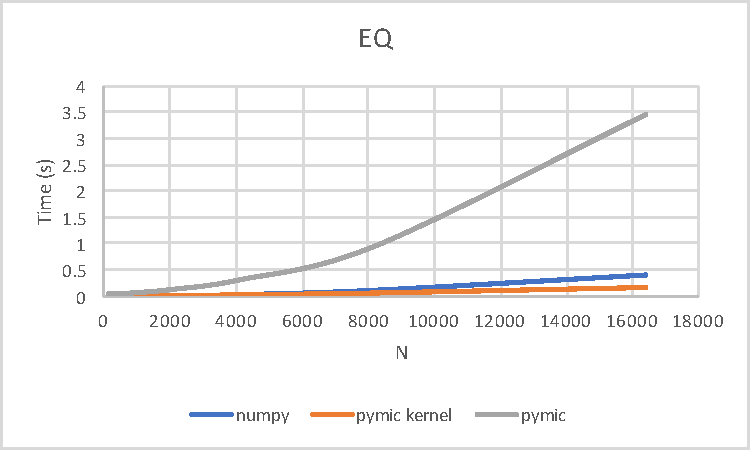
\includegraphics[scale=0.5]{img/group1/eq.pdf}
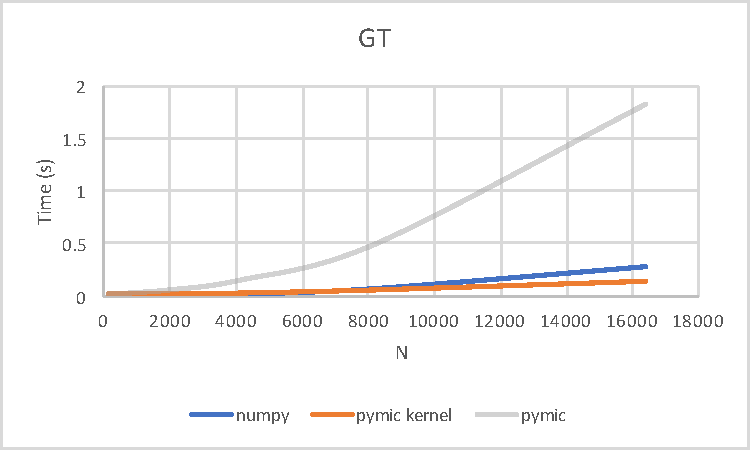
\includegraphics[scale=0.5]{img/group1/gt.pdf}
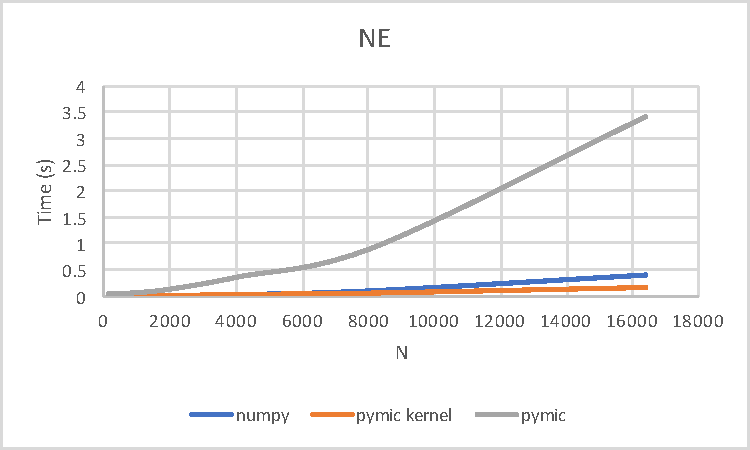
\includegraphics[scale=0.5]{img/group1/ne.pdf}
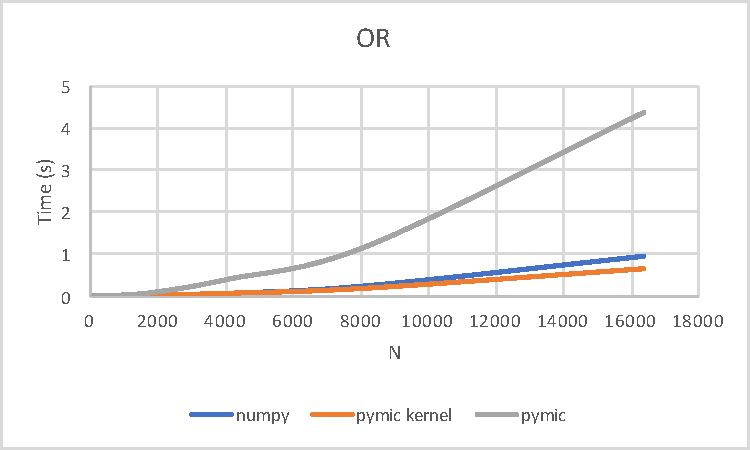
\includegraphics[scale=0.5]{img/group1/or.pdf}
\caption{Benchmark of group 1}
\label{fig:func-or}
\end{figure}

%\begin{table}[]
%\centering
%\caption{Time execution of Group 1}
%\label{tab:group1}
%\resizebox{\textwidth}{!}{\begin{tabular}{|c|c|c|c|c|c|c|c|c|c|c|c|}
%\hline
%
%\multirow{13}{*}{Group 2} 	& Function 	& Size & 128 & 256 & 512 & 1024 & 2048 & 4096 & 8192 & 16384 \\ \cline{2-11}
%
%\multirow{13}{*}{} 			& \multirow{3}{*}{EQ} 	& Numpy & 0.00004 & 0.00006 & 0.00019 & 0.00065 & 0.00532 & 0.02188 & 0.10596 & 0.39615\\
%\multirow{13}{*}{} 			& \multirow{3}{*}{} 		& PyMIC kernel & 0.02835 & 0.03057 & 0.02829 & 0.0284 & 0.03016 & 0.04298 & 0.07092 & 0.15468 \\
%\multirow{13}{*}{} 			& \multirow{3}{*}{} 		& PyMIC & 0.03565 & 0.03695 & 0.03747 & 0.05694 & 0.11581 & 0.29955 & 0.94572 & 3.46047 \\ \cline{2-11}
%
%\multirow{13}{*}{} 			& \multirow{3}{*}{GT} 	& Numpy & 0.00003 & 0.00007 & 0.00029 & 0.00111 & 0.00385 & 0.01717 & 0.07109 & 0.28695 \\
%\multirow{13}{*}{} 			& \multirow{3}{*}{}	 	& PyMIC kernel & 0.02772 & 0.02794 & 0.0277 & 0.02795 & 0.02828 & 0.03334 & 0.06056 & 0.13563\\
%\multirow{13}{*}{} 			& \multirow{3}{*}{} 		& PyMIC & 0.03008 & 0.03143 & 0.03248 & 0.04231 & 0.06886 & 0.15801 & 0.49964 & 1.82656\\ \cline{2-11}
%
%\multirow{13}{*}{} 			& \multirow{3}{*}{NE} 	& Numpy & 0.00003 & 0.00006 & 0.0003 & 0.00069 & 0.00592 & 0.02441 & 0.10494 & 0.42276\\
%\multirow{13}{*}{} 			& \multirow{3}{*}{}	 	& PyMIC kernel & 0.02768	& 0.02471 & 0.02796 & 0.02835 & 0.02826 & 0.04767 & 0.07064 & 0.16073 \\
%\multirow{13}{*}{} 			& \multirow{3}{*}{} 		& PyMIC & 0.03313 & 0.03069 & 0.0371 & 0.05222 & 0.12364 & 0.35599 & 0.92778 & 3.42537\\ \cline{2-11}
%
%\multirow{13}{*}{} 			& \multirow{3}{*}{OR} 	& Numpy & 0.00008 & 0.00032 & 0.00045 & 0.00254 & 0.01586 & 0.06144 & 0.24561 & 0.97365\\
%\multirow{13}{*}{} 			& \multirow{3}{*}{}	 	& PyMIC kernel & 0.02784 & 0.02825 & 0.03033 & 0.03554 & 0.04832 & 0.08806 & 0.20858 & 0.66821\\
%\multirow{13}{*}{} 			& \multirow{3}{*}{} 		& PyMIC & 0.03524 & 0.03544 & 0.03951 & 0.05648 & 0.1325 & 0.42557 & 1.20206 & 4.36309\\ \hline
%
%\end{tabular} }
%\end{table}

\subsubsection{Group 2}
%The second group consists of functions of arithmetic, exponent and logarithm. As usually, pymic line is the slowest. The two other lines can be almost equal, or one can run faster than another and vice versa. For better clarification. We will have three subgroup.
%
%\begin{itemize}
%\item In subgroup 1, the pymic kernel line is approximately equal to numpy. It consists of 9 functions
%
%\item The next subgroup consist 5 functions that runs faster than those of numpy. In arange graph, at first numpy achieves better result than pymic kernel, but when N is getting larger, pymic starts to catch up and runs faster than numpy. The benchmark results of function exp and log are quite interesting, pymic line in exp is almost equal when N is less than 6000, while pymic line in log graph is much faster than numpy. The reason is that for functions such as exponent and logarithm, Intel Compiler includes a mathematical software library containing highly optimized and very accurate mathematical functions, commonly used in scientific or graphic applications [https://software.intel.com/en-us/node/522653].
%
%
%\item Finally,we have three functions that do not run as good as numpy functions. Although, when N gets bigger than N 7500, they starts to works as efficiently as those of numpy.  
%\end{itemize}
%%%%%%%%%%
The second group consists of functions of arithmetic, exponent and logarithm. As usual, pymic line of most functions is the slowest, but when N is getting larger, pymic starts to work more efficient and runs faster than numpy. However, there are still some exceptional functions:

\begin{figure}
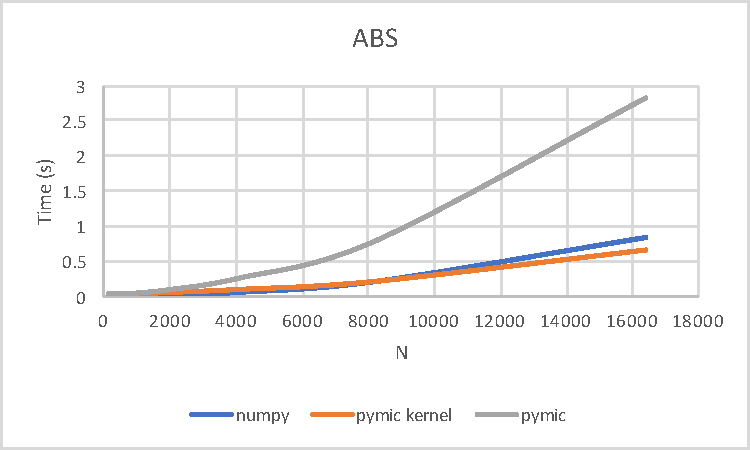
\includegraphics[scale=0.5]{img/group2/abs.pdf}
\includegraphics[scale=0.5]{{"img/group2/argmax axis1"}.pdf}
\end{figure}

\begin{figure}
\centering
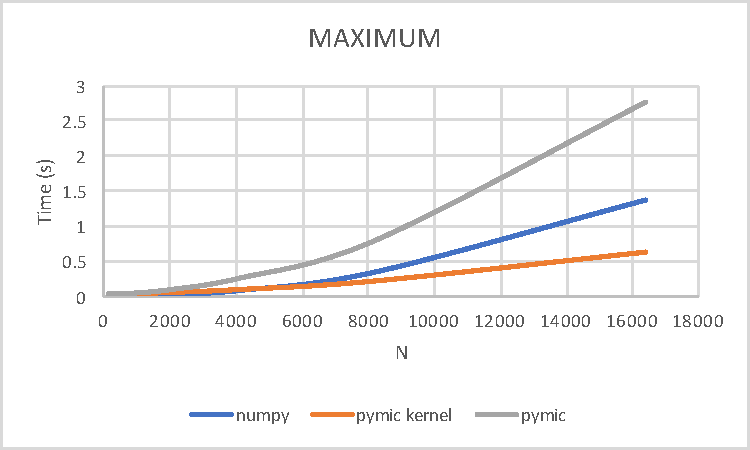
\includegraphics[scale=0.5]{img/group2/maximum.pdf}
\end{figure}

\begin{figure}[]
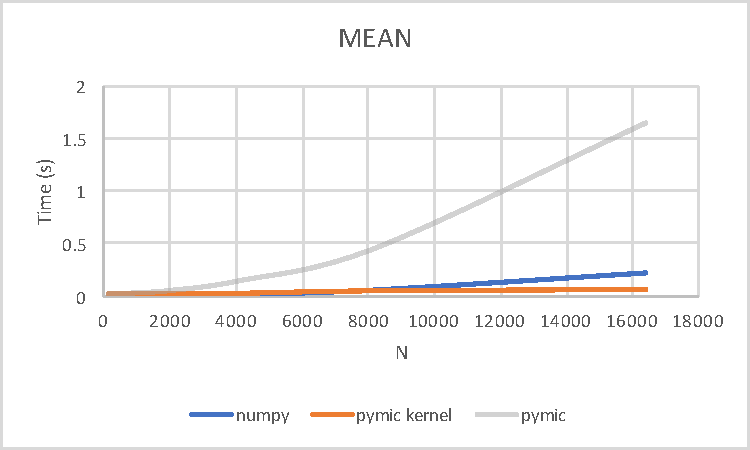
\includegraphics[scale=0.5]{img/group2/mean.pdf}
\includegraphics[scale=0.5]{{"img/group2/sum axis0"}.pdf}
\end{figure}

\begin{figure}[]
\includegraphics[scale=0.5]{{"img/group2/sum axis1"}.pdf}
\includegraphics[scale=0.5]{{"img/group2/sum axisNone"}.pdf}
\end{figure}

\begin{figure}[]
\includegraphics[scale=0.5]{{"img/group2/add same shape"}.pdf}
\includegraphics[scale=0.5]{{"img/group2/add diff shape"}.pdf}
\end{figure}

\begin{figure}[]
\includegraphics[scale=0.5]{{"img/group2/sub same shape"}.pdf}
\includegraphics[scale=0.5]{{"img/group2/sub diff shape"}.pdf}
\end{figure}

\begin{figure}[]
\includegraphics[scale=0.5]{{"img/group2/mul diff shape"}.pdf}
\includegraphics[scale=0.5]{{"img/group2/mul same shape"}.pdf}
\end{figure}

\begin{itemize}
	\item Function ARGMAX axis=0
	\item Fucntion ARANGE
	\item Function EXP and LOG
\end{itemize}

In function ARANGE, pymic line and numpy are approximately the same because it requires no data transferred to coprocessor. Beside function ARANGE, the numpy line of all functions mentioned above is slower than pymic line which includes transferring time. The results of function EXP and LOG can be explained that for exponential and logarithmic functions, Intel Compiler includes a mathematical software library containing highly optimized and very accurate mathematical functions, commonly used in scientific or graphic applications \cite{mathlib}.

\begin{figure}[]
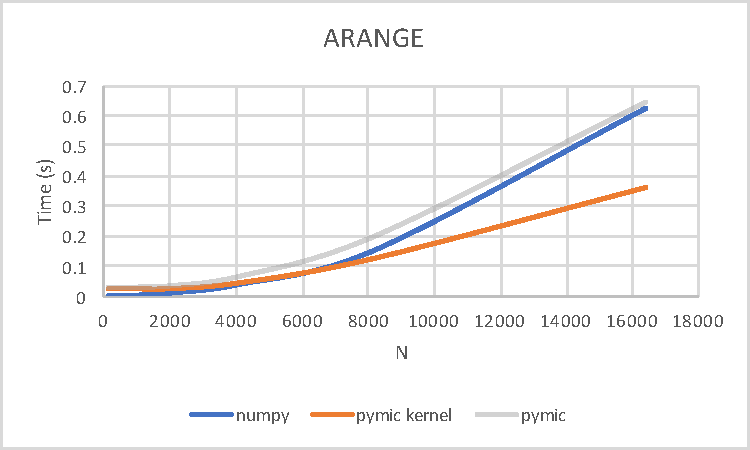
\includegraphics[scale=0.5]{img/group2/arange.pdf}
\includegraphics[scale=0.5]{{"img/group2/argmax axis0"}.pdf}
\end{figure}

\begin{figure}[]
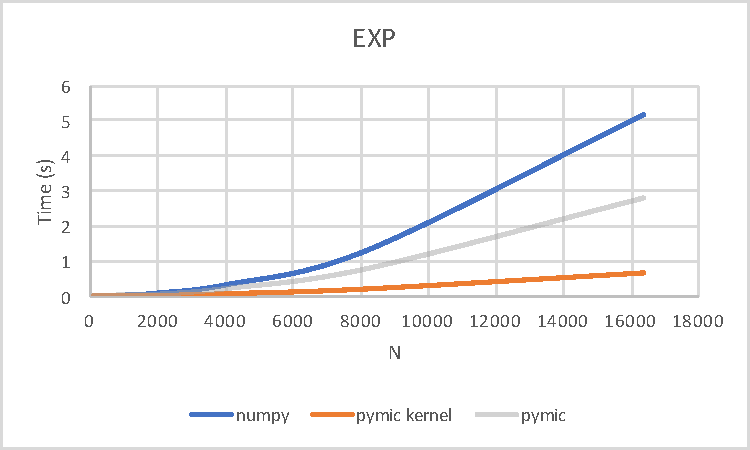
\includegraphics[scale=0.5]{img/group2/exp.pdf}
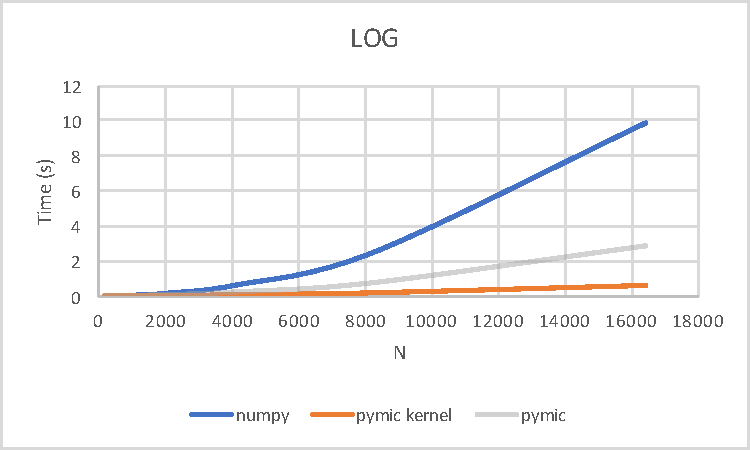
\includegraphics[scale=0.5]{img/group2/log.pdf}
\end{figure}

\subsubsection{Group 3}
In the final group, we use FLOPS (floating point operation per second) for matrix multiplication benchmark instead of time so that we can know how faster this function can achieve in comparison to theoretical performance. This function in pymic will call one of functions of Intel Math Kernel Library (MKL). General matrix multiplication of Intel MKL has been optimized for Intel architecture and proved the efficiency even for small size. 

In Fig. \ref{fig:func-dot}, we can see that peak performance of numpy, pymic kernel and pymic lines are 574, 849 and 596 GLOPS respectively. For small size matrix, numpy works more efficiently than pymic kernel, but pymic kernel starts to outperform numpy when N is greater than 2500. As pymic kernel, pymic also runs faster than numpy when N is greater than 13000. The computation time of pymic can compensate its transferring time, which leads to better performance than Numpy. Moreover, without including transferring overhead, pymic kernel runs 200 GFLOPS faster than pymic

\begin{figure}[]
\centering
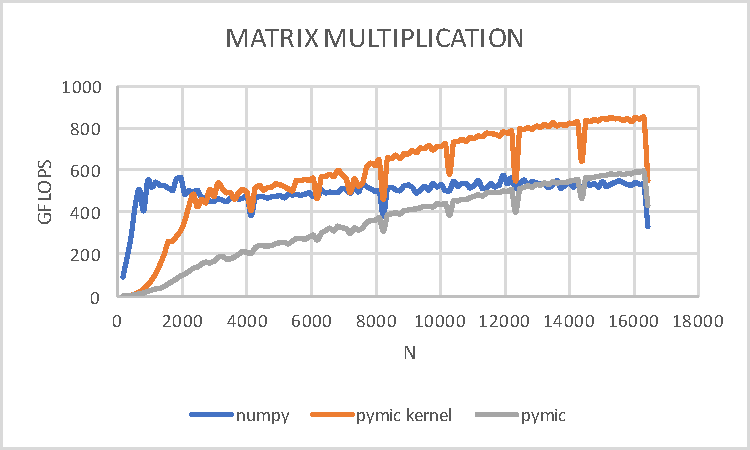
\includegraphics[scale=0.7]{img/dot128.pdf}
\caption{Matrix Multiplication}
\label{fig:func-dot}
\end{figure}

%%%% TRI %%%
\subsection{Chainer-MNIST}
%
The intention of this section is to evaluate the performance of a handwritten digit recognition application that uses pyMIC2 to perform parts of computation on Intel Xeon Phi coprocessor. Our experimental evaluation focuses on two aspects. The first one is the different between CPU and coprocessor computing capabilities, the other one is the potential of using pyMIC2 in deep learning applications.
\subsubsection{Chainer-numpy:}
%
Chainer is a well-known framework for Artificial Neural Network(ANN). One of its advantages is flexibility, which enables its users to create complex architectures simply and intuitively. Similar to TensorFlow, Caffe or Theano, Chainer uses backpropagation algorithm \cite{backprop} for training data and adjusting network's parameters. However, by using "Define-by-Run" scheme,  the network is defined on-the-fly while running actual forward computation, it makes an network created by Chainer become easier to debug than other frameworks. Therefore, an application written by Chainer integrated pyMIC2 has a faster development time.
%

\subsubsection{Experimental Setup:}
%

Our experiments are performed on a combination of CPU Intel Xeon E5 and Intel Xeon Phi 7120P coprocessor. The technical specifications of our system are described in Table \ref{tab:sys-spec} . The framework is compiled for coprocessor using Intel compiler version 17.0.4 as well as OpenMP parallel programming API implementation by Intel  and MKL [*]version. All measurements are carried out 100 times and averaged to eliminate variances in the resulting measurements.
%
\begin{table}[]
\centering
\caption{Hardware specifications}
\label{tab:sys-spec}
\begin{tabular}{|c|c|c|}
\hline
\textbf{Codename} 	& \textbf{CPU} 	& \textbf{Coprocessor} \\ \hline
\textbf{Model} & Intel Xeon E5-2680V3  & Intel Xeon Phi 7120P \\
\textbf{Microarchitecture} & Sandy Bridge EP & Intel Many Integrated Core \\
\textbf{Clock frequency} & 2.50/3.30 GHz & 1.24/1.33 GHz \\
\textbf{Memory Size} & 512 GB & 16 GB \\
\textbf{Cache} & 30.0 MB SmartCache & 30.5 MB L2 \\
\textbf{Max Memory Bandwidth} & 68 GB/s & 352 GB/s\\
\textbf{Core/Threads} & 12/24 & 61/244 \\
\hline
\end{tabular} 
\end{table}


We evaluate our approach using the MNIST \cite{mnist} dataset of handwritten digits including training set of 60,000 examples,  and 10,000 test images, each image contains 28x28 pixel grey levels. The architecture of testing ANNs has 1000, 1500, 2000, 2500 ... 5500 units, each unit represents a node in the network's hidden layer. In order to simplify the performance evaluation process, we just modify the ANNs with one hidden layer, which means our ANNs have only 3 layers which are input, output and hidden. Detailed information of the ANNs used in our evaluation are shown in Table \ref{tab:ann-info}.
%
\begin{table}[]
\centering
\caption{ANN architecture}
\label{tab:ann-info}
\begin{tabular}{|c|c|}
\hline
\multicolumn{2}{|c|}{\textbf{ANN Configuration}}\\ \hline
\textbf{Layer} 	& 3 \\
\textbf{Batch Size} & 60000 \\
\textbf{Connetion Function} & Linear  \\
\textbf{Activation Function} & Relu  \\
\textbf{Loss Function} & Softmax Cross Entropy \\
\textbf{Gradient Method} &  Stochastic gradient descent \\
\hline
\end{tabular} 
\end{table}
\subsubsection{Result:}
%
We perform entire evaluation on Docker \cite{docker} in order to easily customize the constraints of system resources. A simple experiment is conducted to ensure that the execution of the ANNs in Docker is similar to physical machine and we obtain the expected result. Thereafter, we start to evaluate the performance of applications, written by two versions of Chainer, one is original version and the other is pyMIC2 integrated version, called Chainer-XP, to execute on Intel Xeon Phi coprocessor.

\begin{figure}[]
\centering
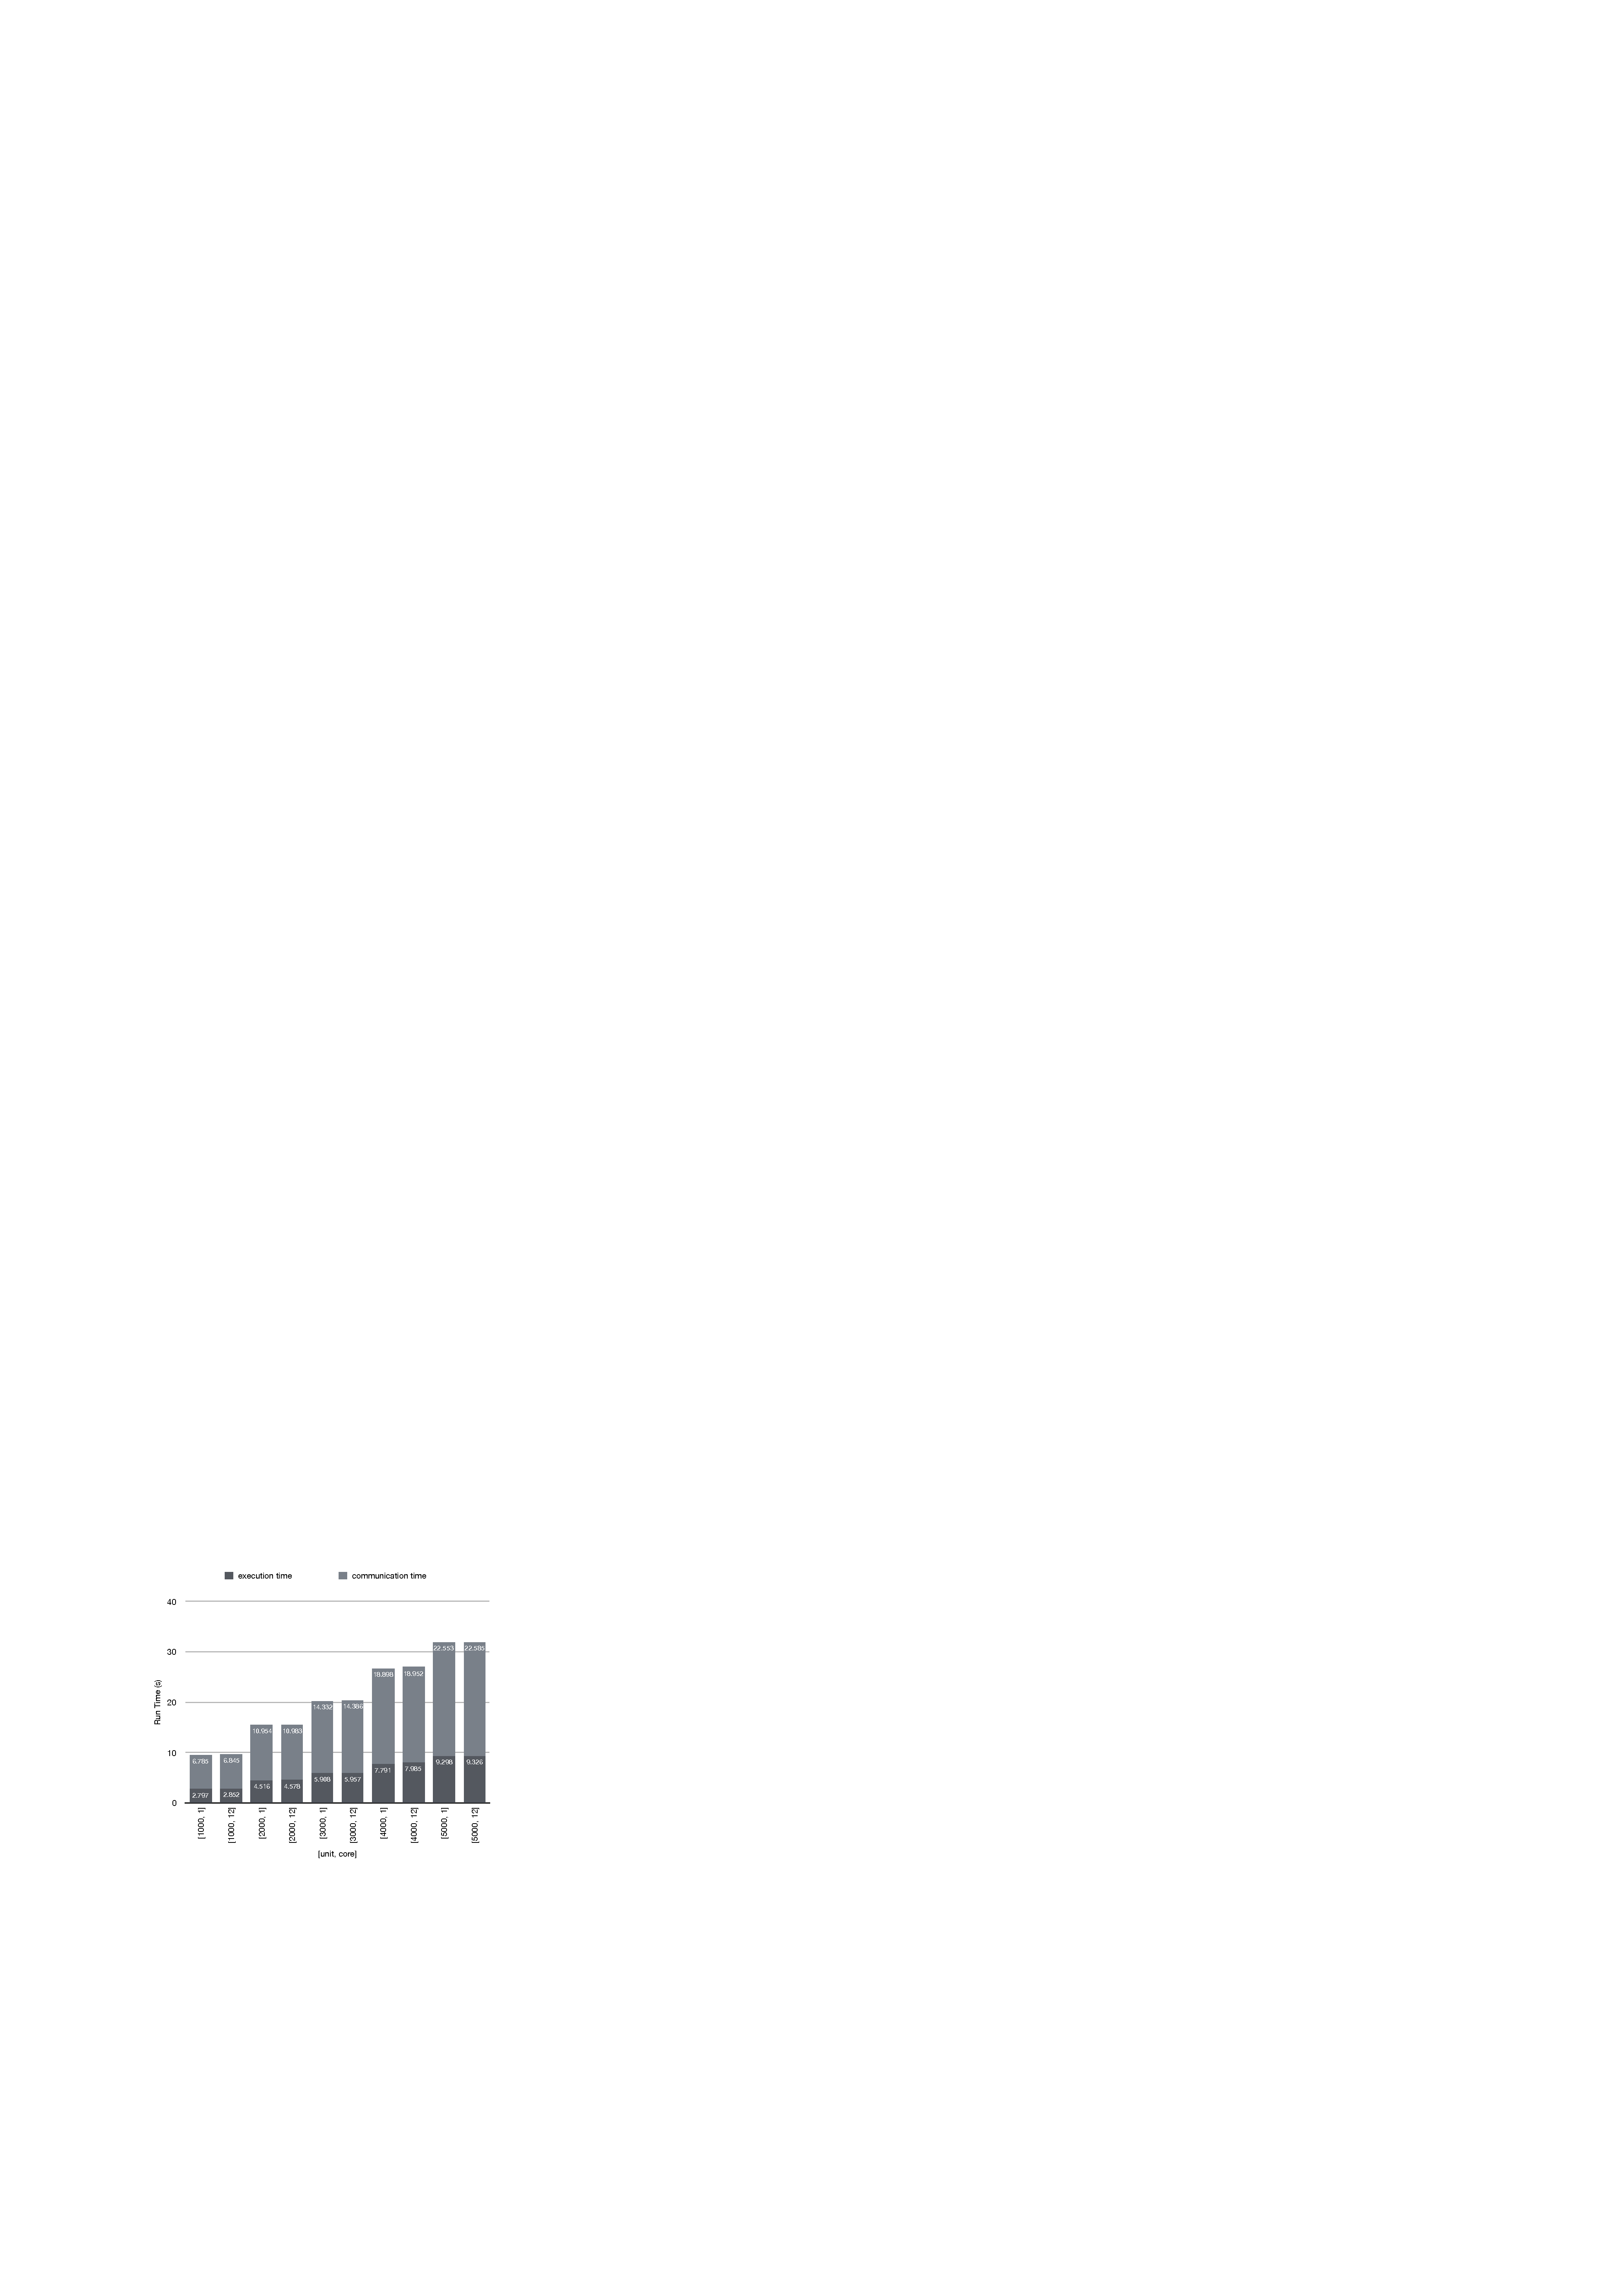
\includegraphics[scale=0.6]{img/a.pdf}
\caption{Chainer-XP sigle core and full core}
\label{fig:1-core-and-full-core}
\end{figure}

Results presented for Chainer-XP in Figure \ref{fig:1-core-and-full-core} show that all experiments of our ANNs training corresponding to the number of units: 1000, 2000, 3000, 4000 and 5000, are executed in roughly equal time periods without being influenced by the number of CPU cores. That also means most of the computational functions have been offloaded into Intel Xeon Phi coprocessor. Moreover, it can be seen that the data communication occupies most of the execution time of training process, overhead is caused by the synchronization between CPU(host) and coprocessor(device) during the calculation. Overall, pyMIC2 is a potential framework which supports its users run ANNs entirely on Intel Xeon Phi. However, the synchronization occupies a prominent role throughout the training process, if it is not tightly controlled, the performance can be devastatingly reduced.


In this experiment, we evaluate pyMIC2's computational capabilities in Intel Xeon Phi. The first ANN (ANN-1) written by original Chainer is executed on a Docker that used full core of a CPU Intel Xeon E5, and the other ANN(ANN-2) written by Chainer-XP on a Docker used only one core combined with Intel Xeon Phi coprocessor. In detail, both ANNs contain three layers and 1000 units in hidden layer, the network's configuration details are described in the Table \ref{tab:ann-info}. Then we measure thoroughly the computation time of all functions during training process and find out that with the second ANN calculation time on coprocessor occupies just approximately 29.2\% total run time. More specifically, with a mentioned ANN, the calculation is mainly executed in \textit{dot} function, about 90.2\% of computation time as it is called three times each training.
\begin{figure}[]
\centering
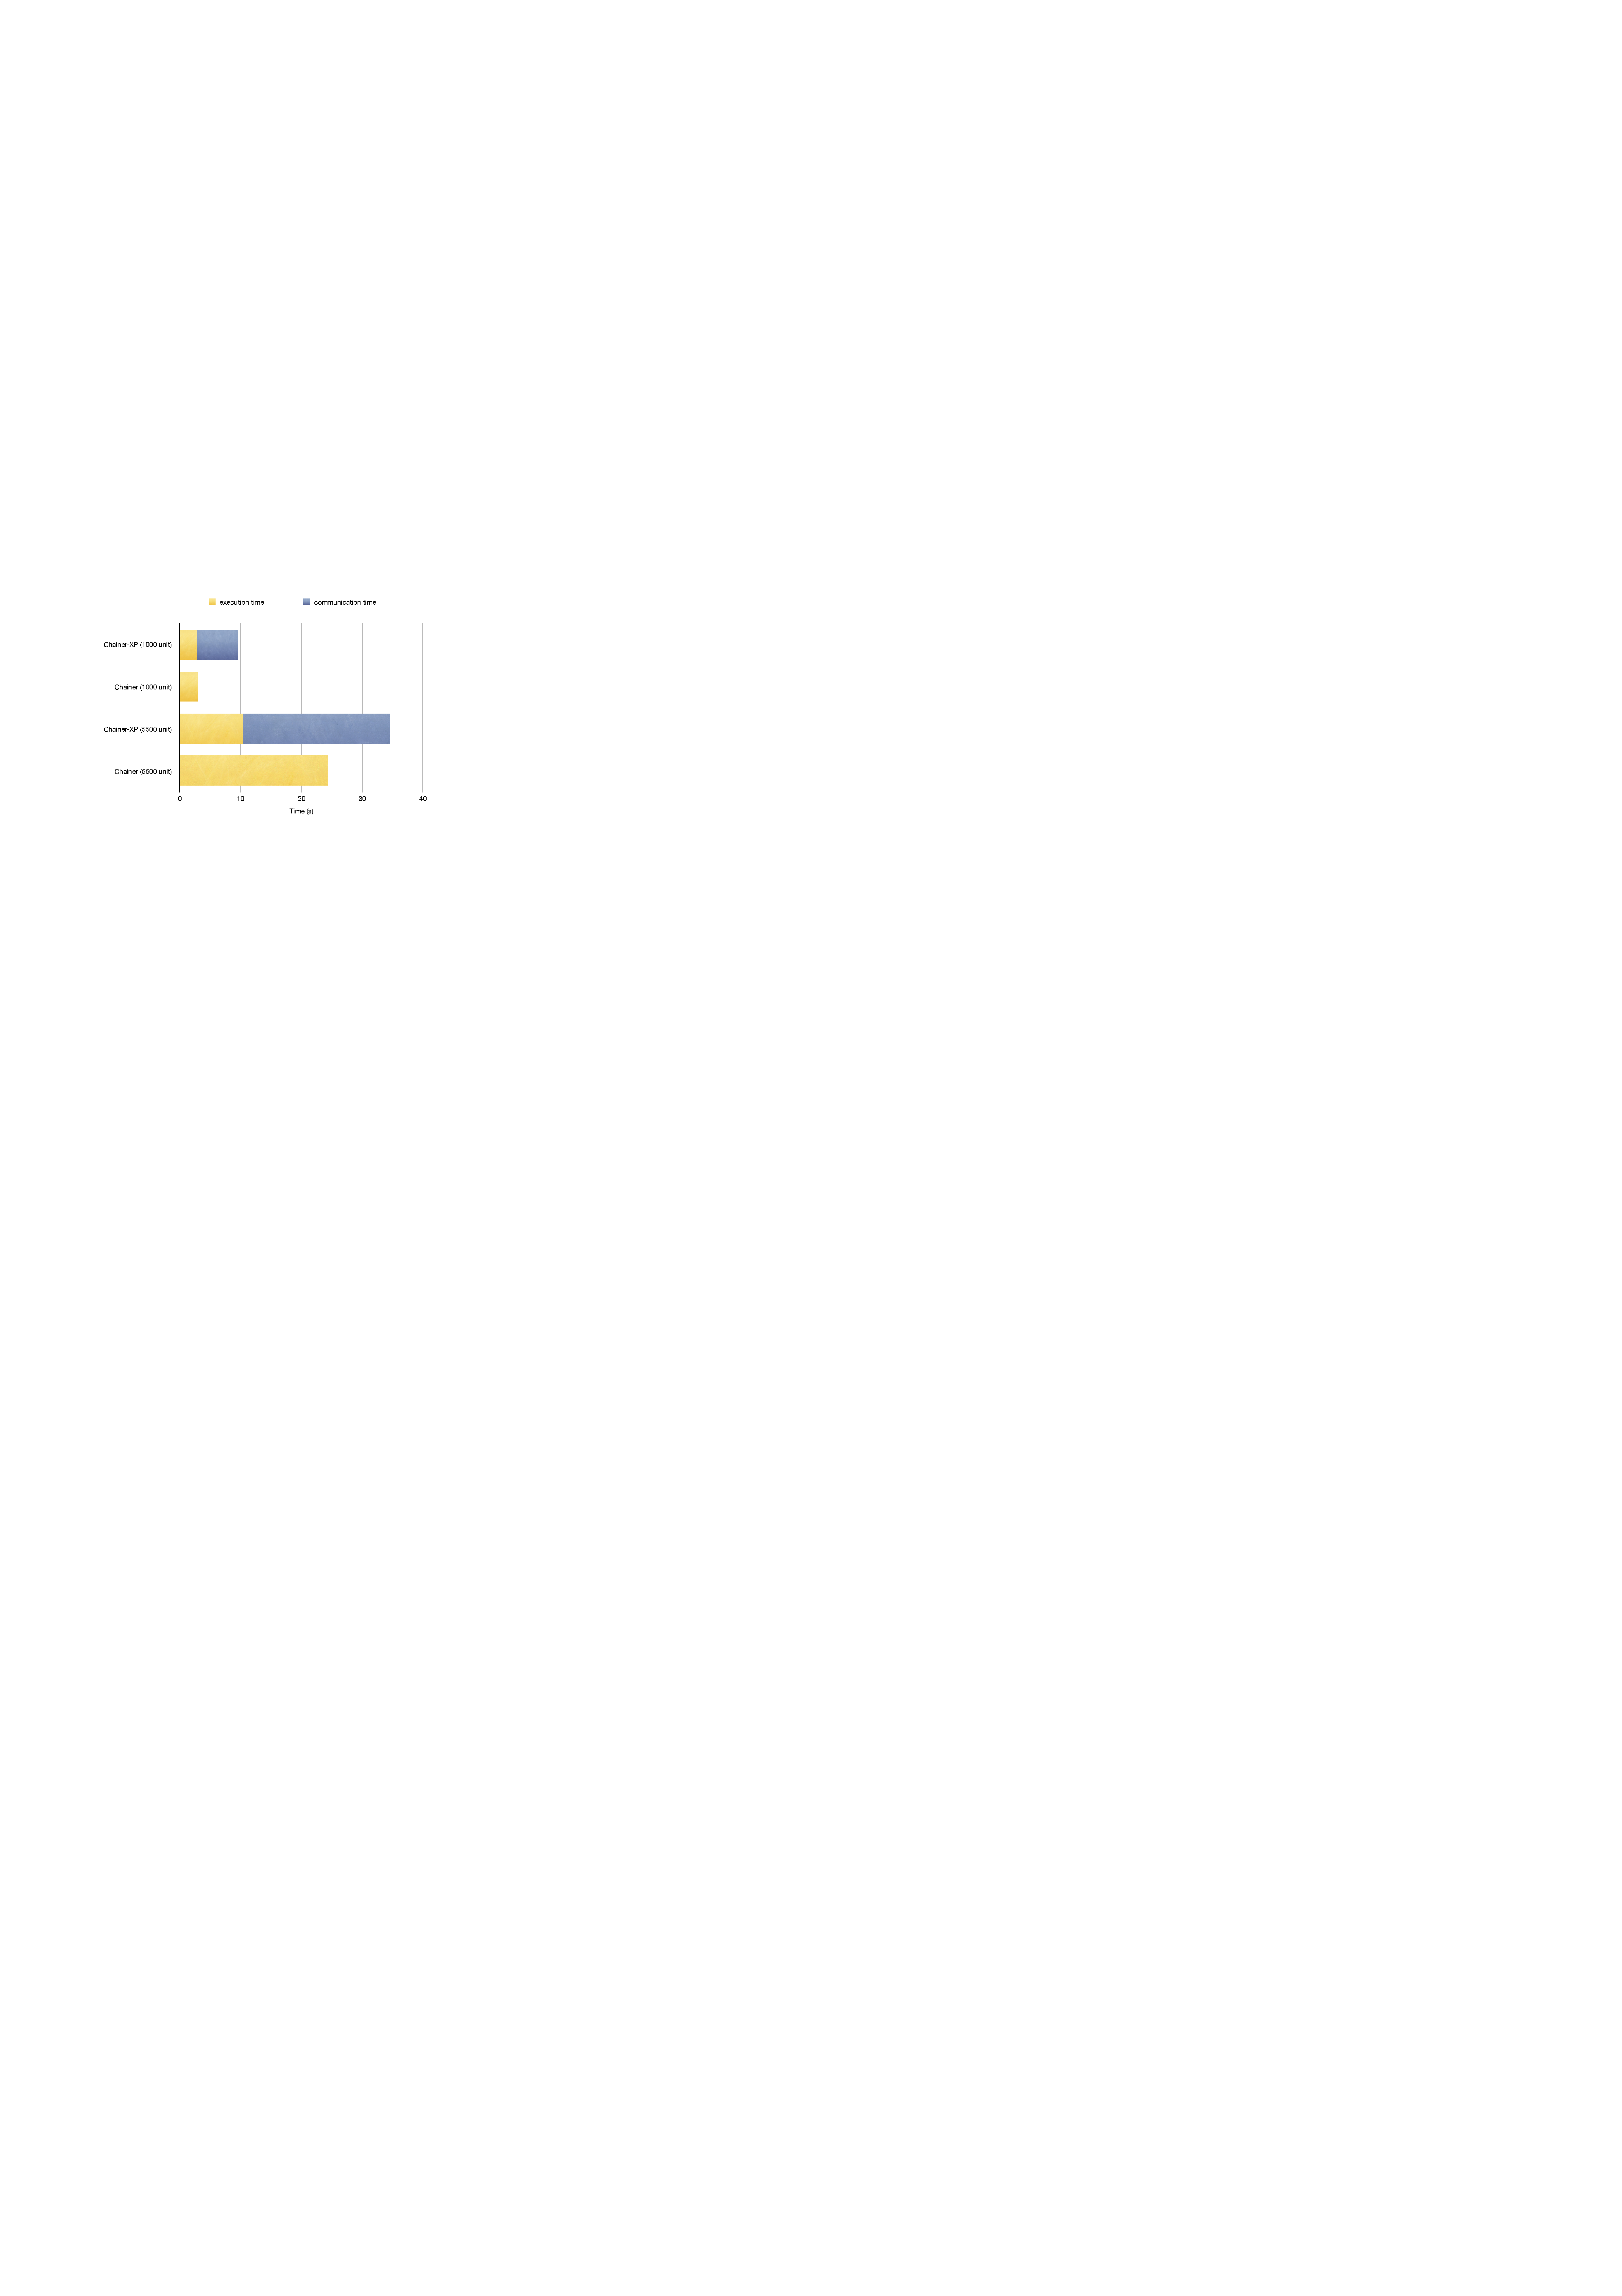
\includegraphics[scale=0.5]{img/b.pdf}
\caption{Chainer-XP single core and 12 core}
\label{b.pdf}
\end{figure}

The biggest matrix size that the \textit{dot} function must perform during the execution of the above network is [784,60000] x [60000,1000], which corresponds to 70.8\% total run time used to synchronize data between host and device. Although the purely computation time of ANN-2 on the coprocessor is approximately 1.93 times faster, the total training time was about 1.78 times slower than ANN-1 on the full core CPU. The reason for this drop in performance is transmitting data between hosts and devices repeatedly leading to overlap and redundancy. However, the cause of this result is that the pyMIC2 integration into Chainer has not been optimized, therefore, we can significantly improve the result as pyMIC2 provides objects and functions that strictly support memory allocation and deallocation on Intel Xeon Phi coprocessor. In other words, we must fully understand how Chainer organizes the data so that we can reduce the communication between host and device and increase the performance of training process. As mentioned above, in this paper we just focus on the computing capabilities; thus, in the rest of the experiment, the number of units is raised to 5500 with the aim of increasing the size of the largest matrix to [784,60000] x [60000,5500]. The observed result shows that the ratio between computation time on coprocessor and total training time is almost unchanged at about 30\%. In addition, when the size of one of the two \textit{dot} operands expanded 5.5 times, the computation time on the Intel Xeon Phi increased only 3.8 times, while the CPU run time is grown up to 7.8 times, and total training time achieve 1.2 times faster than CPU. Thus, with several medium configuration CPUs, there is the possibility that we can speed up with Intel Xeon Phi for large-scale computing in ANNs.
\begin{figure}[]
\centering
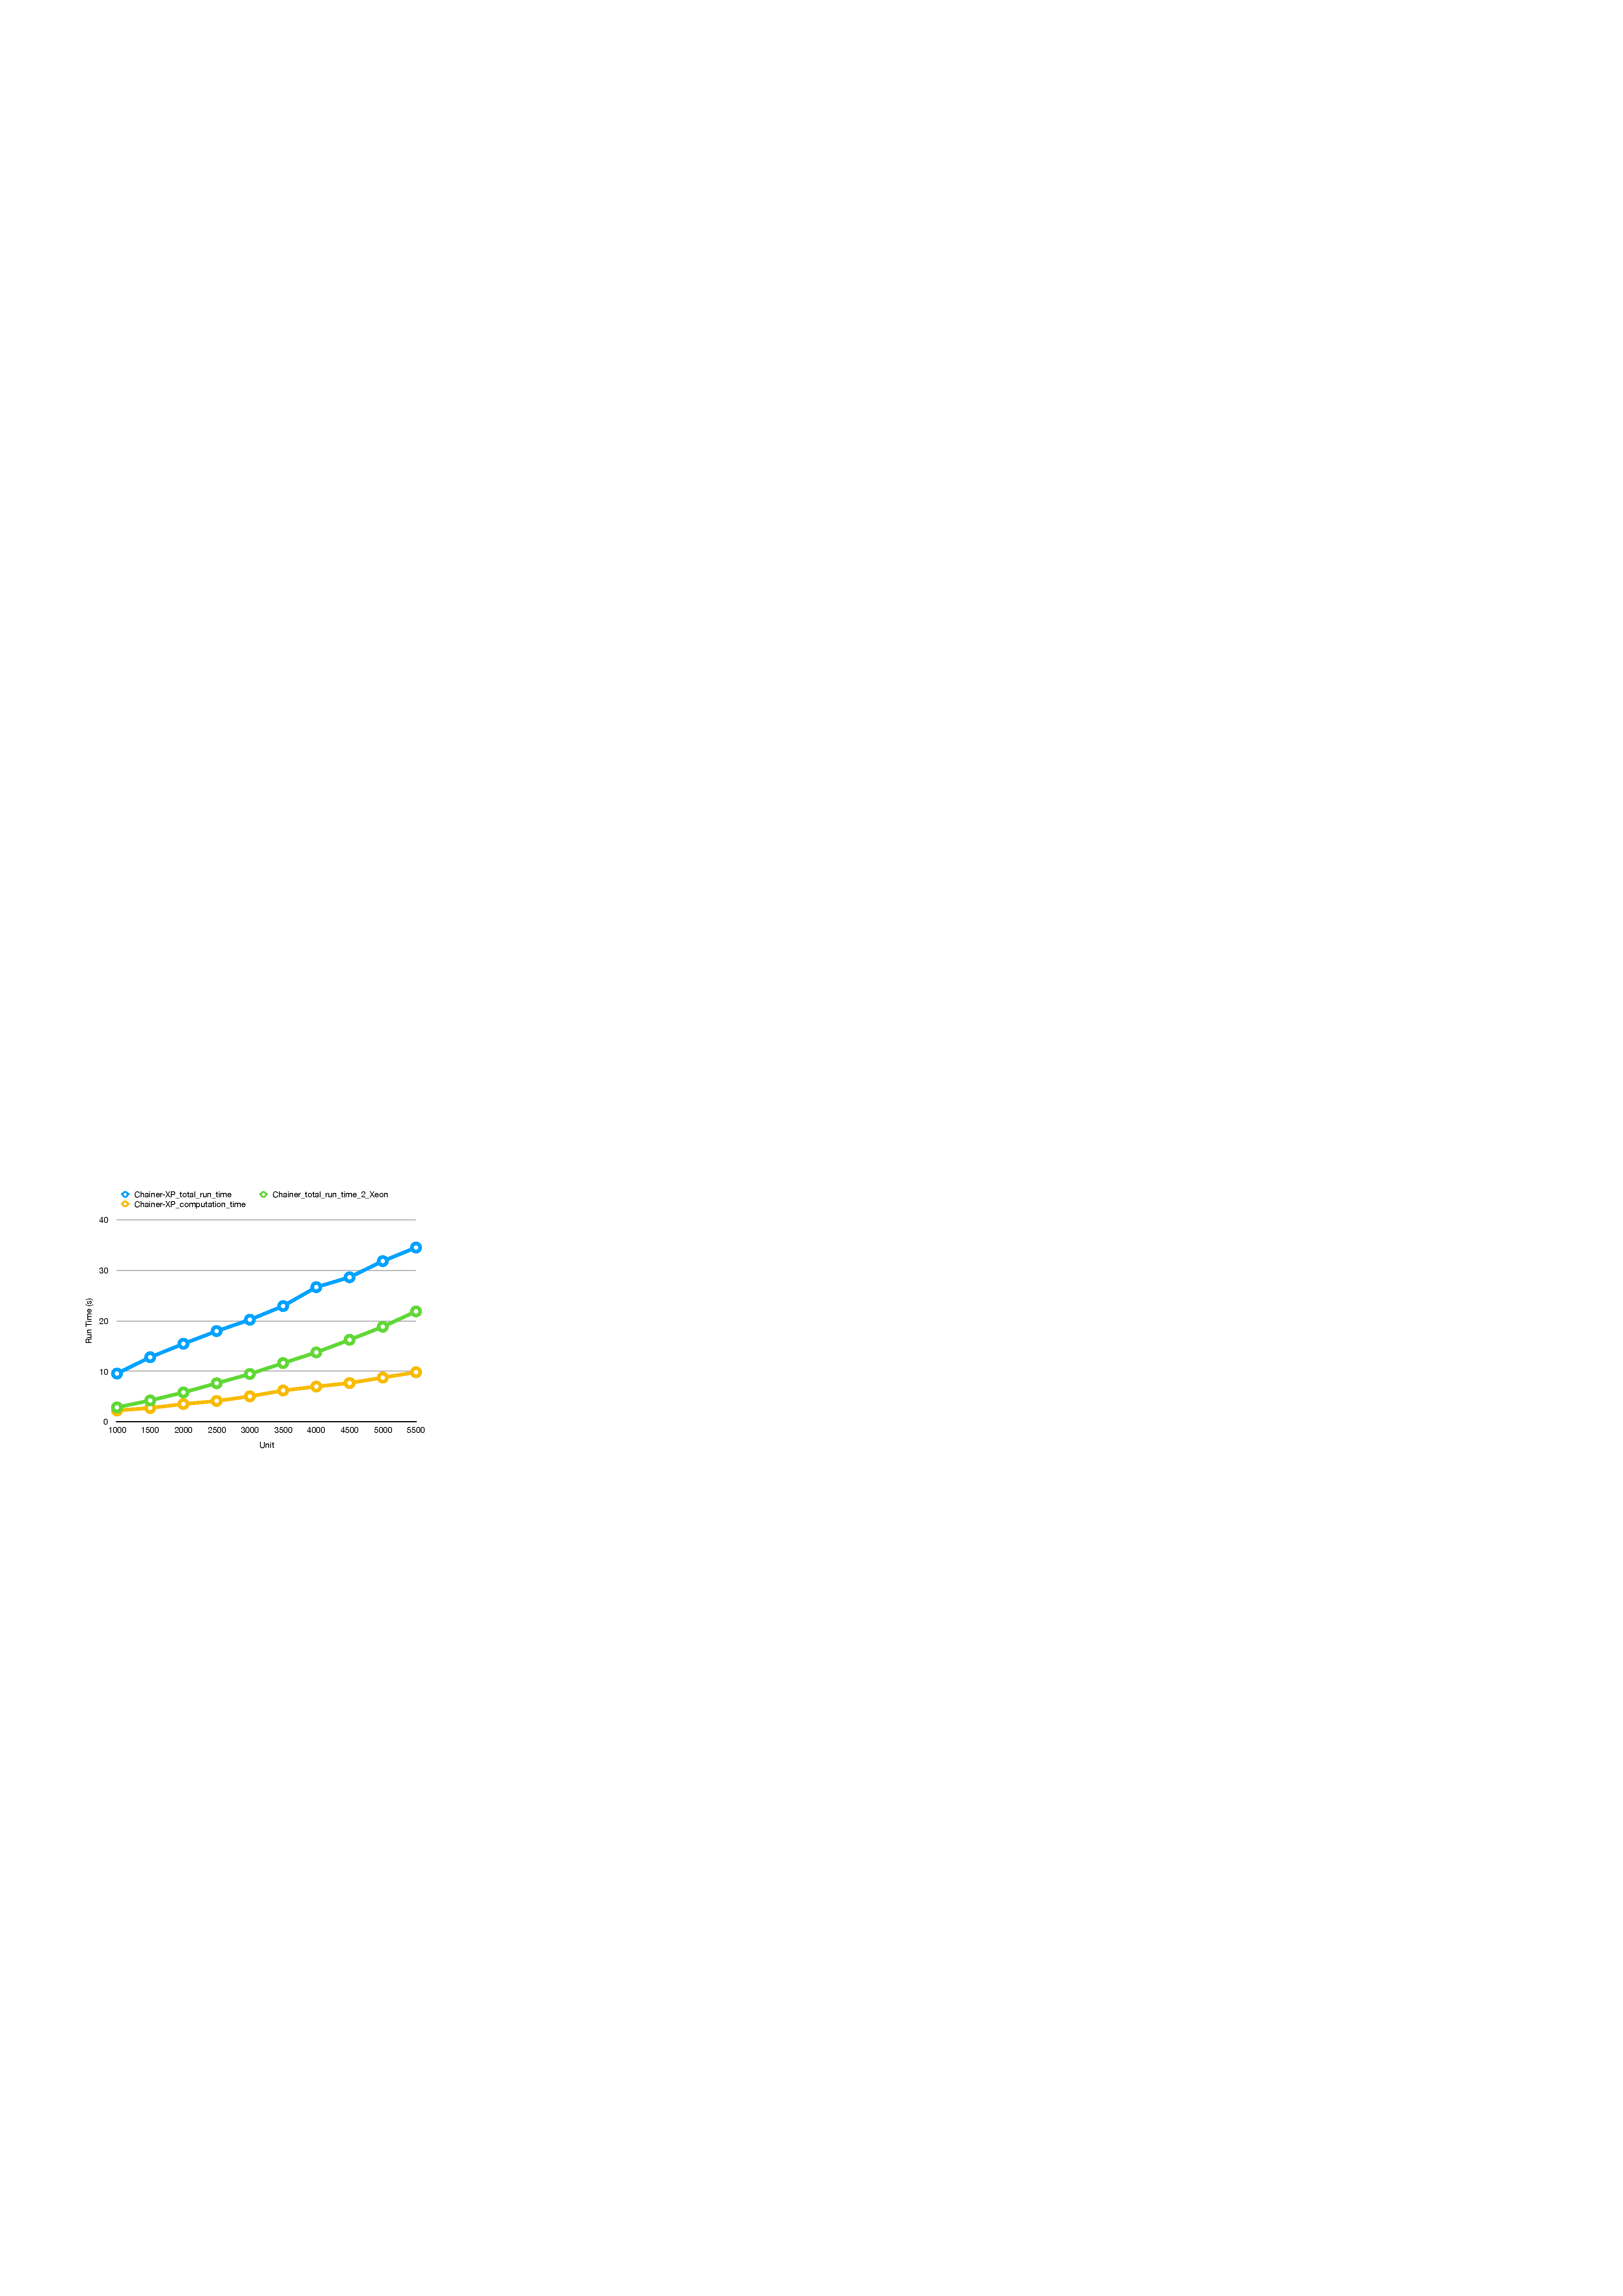
\includegraphics[scale=0.6]{img/c.pdf}
\caption{Chainer-XP vs Chainer}
\label{chainer-xp-vs-chainer}
\end{figure}

The comparison between two versions of Chainer is illustrated in Figure \ref{chainer-xp-vs-chainer}. In order to obtain this experience, The ANN-1 is executed entirely on CPU with a Docker containing dual-processor Intel Xeon E5, which has computing capability approximately 960 GFLOP/s, while the peak performance of an Xeon Phi coprocessor is approximate 1 TFLOP/s \ref{halyo2014first} in double precision. Although they almost have the similar processing power, computation time of an ANN integrated pyMIC2  is getting faster and faster than this ANN which runs in CPU. Hence, It can be seen that pyMIC2 has used the Xeon Phi's SIMD mechanism, as well as Vectorization technique of Intel Xeon Phi quite effectively in calculating sequential elements.

%%%%%%%%%%%%

\section{Discussion, 1page}
discussion.tex

\section{Conclusions and Future Work, 1 page}
\label{conclusion}
In this article, we propose and develop pyMIC2 which is a NumPy-like library for deep learning frameworks run on Intel Xeon Phi Knights Corner coprocessor. This library is an extension of pyMIC that is a Python offloading module for Intel Xeon Phi Knights Corner coprocessor. The experimental results show that pyMIC2 not only outperforms compared with NumPy when considering them on two distinct hardware platforms with the theoretical performance, is but also able to be highly integrated into one popular deep learning framework Chainer with convincing performance. 

However, pyMIC2 still contains several limitations. First, we initially implement some fundamental functions which are sufficient to integrate it into Chainer in order to run ANNs with MNIST dataset. There are still enormous functions that need to be implemented to be capable of running other networks. As a result, we intend to implement other NumPy-like functions so as to apply to other deep learning networks. Second, pyMIC2 can currently be run on at most one Intel Xeon Phi Knights Corner coprocessor and hence, it does still not exploit fully systems containing more than one Intel Xeon Phi Knights Corner coprocessor. For that reason, we intend to enhance pyMIC2 so that it is able to be run such systems. Eventually, computation loads are performed completely on only Intel Xeon Phi coprocessor when using pyMIC2. Central Processing Units (CPUs) have still not been utilized to share the burden of on computation. Therefore, we intend to improve pyMIC2 so that it can be run on both CPUs and the coprocessor simultaneously to boost program performance. 

\bibliographystyle{splncs03}
\bibliography{refs}
%
% ---- Bibliography ----
%
%\begin{thebibliography}{}
%%
%\bibitem[1980]{2clar:eke}
%Clarke, F., Ekeland, I.:
%Nonlinear oscillations and
%boundary-value problems for Hamiltonian systems.
%Arch. Rat. Mech. Anal. 78, 315--333 (1982)
%
%\bibitem[1981]{2clar:eke:2}
%Clarke, F., Ekeland, I.:
%Solutions p\'{e}riodiques, du
%p\'{e}riode donn\'{e}e, des \'{e}quations hamiltoniennes.
%Note CRAS Paris 287, 1013--1015 (1978)
%
%\bibitem[1982]{2mich:tar}
%Michalek, R., Tarantello, G.:
%Subharmonic solutions with prescribed minimal
%period for nonautonomous Hamiltonian systems.
%J. Diff. Eq. 72, 28--55 (1988)
%
%\bibitem[1983]{2tar}
%Tarantello, G.:
%Subharmonic solutions for Hamiltonian
%systems via a $\bbbz_{p}$ pseudoindex theory.
%Annali di Matematica Pura (to appear)
%
%\bibitem[1985]{2rab}
%Rabinowitz, P.:
%On subharmonic solutions of a Hamiltonian system.
%Comm. Pure Appl. Math. 33, 609--633 (1980)
%
%\end{thebibliography}
\clearpage
%\addtocmark[2]{Author Index} % additional numbered TOC entry
%\renewcommand{\indexname}{Author Index}
%\printindex
%\clearpage
%\addtocmark[2]{Subject Index} % additional numbered TOC entry
%\markboth{Subject Index}{Subject Index}
%\renewcommand{\indexname}{Subject Index}
%\input{subjidx.ind}
\end{document}
